\section{はじめに}\label{sec:introduction}

%%%%%%%%%%%%%%%%%%%%%%%%%%%%%%%%%
\begin{figure*}[tbp]
  \centering
  \begin{tabular}{ccccccc}
    $t=0$ && $t=1$ && $t=2$ && $t=3$ \\
    \scalebox{0.75}{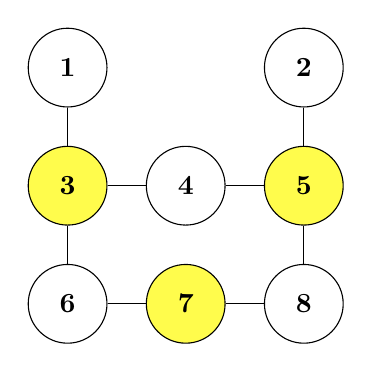
\begin{tikzpicture}[x=1.5cm, y=1.5cm]
  % 設定
  \tikzset{node/.style={circle,draw=black,minimum size=1cm}}
 
  % 色
  \definecolor{yellow}{RGB}{255,251,0}
 
  % 補助線
  % \draw [help lines,blue] (0,0) grid (20,6);
 
  % node %
  \node[node] at (-1,1) (node1) {\textbf{1}};
  \node[node] at (1,1) (node2) {\textbf{2}};
  \node[node, fill=yellow!70] at (-1,0) (node3) {\textbf{3}};
  \node[node] at (0,0) (node4) {\textbf{4}};
  \node[node, fill=yellow!70] at (1,0) (node5) {\textbf{5}};
  \node[node] at (-1,-1) (node6) {\textbf{6}};
  \node[node, fill=yellow!70] at (0,-1) (node7) {\textbf{7}};
  \node[node] at (1,-1) (node8) {\textbf{8}};
 
  \foreach \u / \v in {node1/node3, node2/node5, node3/node4, node3/node6, node4/node5,
    node5/node8, node6/node7, node7/node8}
  \draw (\u) -- (\v);
\end{tikzpicture}
} &
    \lw{$\Rightarrow$} &
    \scalebox{0.75}{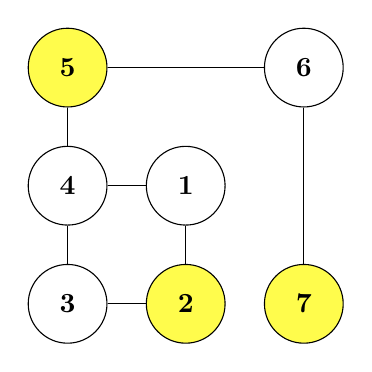
\begin{tikzpicture}[x=1.5cm, y=1.5cm]
  % 設定
  \tikzset{node/.style={circle,draw=black,minimum size=1cm}}
 
  % 色
  \definecolor{yellow}{RGB}{255,251,0}
 
  % 補助線
  % \draw [help lines,blue] (0,0) grid (20,6);
 
  % node %
  \node[node] at (0,0) (node1) {\textbf{1}};
  \node[node, fill=yellow!70] at (0,-1) (node2) {\textbf{2}};
  \node[node] at (-1,-1) (node3) {\textbf{3}};
  \node[node] at (-1,0) (node4) {\textbf{4}};
  \node[node, fill=yellow!70] at (-1,1) (node5) {\textbf{5}};
  \node[node] at (1,1) (node6) {\textbf{6}};
  \node[node, fill=yellow!70] at (1,-1) (node7) {\textbf{7}};
 
  \foreach \u / \v in {node1/node2, node1/node4, node2/node3, node3/node4, node4/node5,
    node5/node6, node6/node7}
  \draw (\u) -- (\v);
\end{tikzpicture}
} &
    \lw{$\Rightarrow$} &
    \scalebox{0.75}{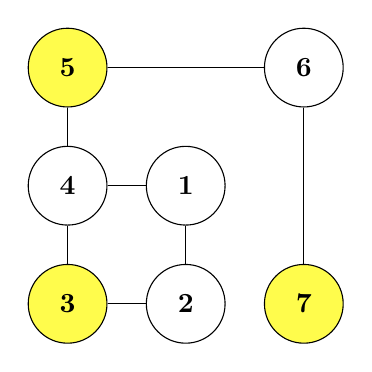
\begin{tikzpicture}[x=1.5cm, y=1.5cm]
  % 設定
  \tikzset{node/.style={circle,draw=black,minimum size=1cm}}
 
  % 色
  \definecolor{yellow}{RGB}{255,251,0}
 
  % 補助線
  % \draw [help lines,blue] (0,0) grid (20,6);
 
  % node %
  \node[node] at (0,0) (node1) {\textbf{1}};
  \node[node] at (0,-1) (node2) {\textbf{2}};
  \node[node, fill=yellow!70] at (-1,-1) (node3) {\textbf{3}};
  \node[node] at (-1,0) (node4) {\textbf{4}};
  \node[node, fill=yellow!70] at (-1,1) (node5) {\textbf{5}};
  \node[node] at (1,1) (node6) {\textbf{6}};
  \node[node, fill=yellow!70] at (1,-1) (node7) {\textbf{7}};
 
  \foreach \u / \v in {node1/node2, node1/node4, node2/node3, node3/node4, node4/node5,
    node5/node6, node6/node7}
  \draw (\u) -- (\v);
\end{tikzpicture}
} &
    \lw{$\Rightarrow$} &
    \scalebox{0.75}{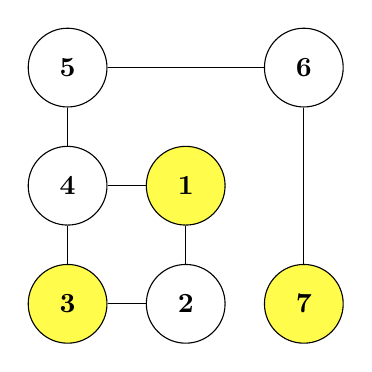
\begin{tikzpicture}[x=1.5cm, y=1.5cm]
  % 設定
  \tikzset{node/.style={circle,draw=black,minimum size=1cm}}
 
  % 色
  \definecolor{yellow}{RGB}{255,251,0}
 
  % 補助線
  % \draw [help lines,blue] (0,0) grid (20,6);
 
  % node %
  \node[node, fill=yellow!70] at (0,0) (node1) {\textbf{1}};
  \node[node] at (0,-1) (node2) {\textbf{2}};
  \node[node, fill=yellow!70] at (-1,-1) (node3) {\textbf{3}};
  \node[node] at (-1,0) (node4) {\textbf{4}};
  \node[node] at (-1,1) (node5) {\textbf{5}};
  \node[node] at (1,1) (node6) {\textbf{6}};
  \node[node, fill=yellow!70] at (1,-1) (node7) {\textbf{7}};
 
  \foreach \u / \v in {node1/node2, node1/node4, node2/node3, node3/node4, node4/node5,
    node5/node6, node6/node7}
  \draw (\u) -- (\v);
\end{tikzpicture}
} \\
    スタート状態 &&&&&& ゴール状態
  \end{tabular}
  \caption{独立集合遷移問題の例}
  \label{fig:ex_isrp}
\end{figure*}
%%%%%%%%%%%%%%%%%%%%%%%%%%%%%%%%%

\textbf{組合せ遷移問題}
(Combinatorial Reconfiguration Problem \cite{%
  core:Heuvel13,core:Nishimura18}
)とは,
基となる組合せ問題とその二つの実行可能解が与えられたとき,
一方から他方へ遷移制約を満たしつつ,
実行可能解のみを経由して到達可能かを判定する問題である.
入力として与えられる二つの実行可能解の片方を
スタート状態,もう一方をゴール状態と呼ぶ.
組合せ遷移問題には様々なバリエーションが存在する.
スタート状態からゴール状態への到達可能性を判定する問題に加え,
最短経路を求める問題,同じ実行可能解を経由しない
(ループのない)最長経路を求める問題などがある.
本稿では,これら三つのバリエーションを,
exsistent, shortest, longest
と呼ぶことにする.

組合せ遷移問題の研究は,最近10年で理論計算機科学の分野を中心に急速に
発展し,理論的な基盤が整備されつつある.
計算複雑性については,基の組合せ問題が NP 完全であるとき,その遷移問題
の多くは PSPACE 完全になることがわかってきている~\cite{core:ItoDHPSUU11}.
代表的な例としては,
命題論理の充足可能性判定問題(SAT),
集合被覆問題,
独立集合,
グラフ彩色問題を基とする組合せ遷移問題などがある~\cite{%
  core:gcp:BonsmaC09,%
  core:gcp:CerecedaHJ11,%
  core:sat:GopalanKMP09,%
  core:ItoDHPSUU11%
}.
%
その一方で,組合せ遷移問題を解く汎用ソルバー,
ヒューリスティックスなど
の実践的な研究開発はまだ始まったばかりである.
今年度から,組合せ遷移に関する国際競技会
CoRe Challenge 2022~\footnote {\tt https://core-challenge.github.io/2022/}
が開催され,今後はソルバー開発を始めとする実践的な研究開発が活発化する
ことが予想される.

\textbf{独立集合遷移問題}
(Independent Set Reconfiguration Problem; ISRP~\cite{core:ItoDHPSUU11})
は,基となる独立集合問題とその二つの実行可能解が与えられたとき,
一方から他方へ遷移制約を満たしつつ,実行可能解のみを経由して到達可能か
を判定する問題である.
独立集合問題は,与えられたグラフ$G$と自然数$k$に対して,$G$が要素数$k$
以上の独立集合をもつかどうかを判定する問題である.
ISRP は,スタート状態の独立集合のすべての頂点にトークン(token)を配置し,
独立集合問題の制約と遷移制約を満たしつつ,トークンをゴール状態に移動で
きるかどうかを判定する問題と考えることもできる.
遷移制約としては,
``1回の遷移で一つのトークンが移動できる (token jumping)''  と
``1回の遷移で一つのトークンが隣接頂点へのみ移動できる (token sliding)'' 
の2種類がよく用いられる.

本稿では,CoRe Challenge 2022 競技会のベンチマーク問題として採用されて
いる token jumping に基づく独立集合遷移問題を対象とする.
独立集合遷移問題の例を図~\ref{fig:ex_isrp}に示す.
この例は,頂点数8,要素数$k=3$の独立集合問題を基としており,
トークン(黄色)がスタート状態からゴール状態へ3ステップで遷移しているこ
とがわかる.

\textbf{解集合プログラミング}
(Answer Set Programming; ASP \cite{%
  Gelfond88:iclp,
  Niemela99:amai,
  Baral03:cambridge,
  Inoue08:jssst})
は,論理プログラミングから派生した宣言的プログラミングパラダイムの一つ
である.
ASP 言語は一階論理に基づく知識表現言語の一種である.
ASP システムは安定モデル意味論に基づく解集合を計算するシステムである.
近年,SAT 技術~\cite{Knuth:TAOCP:SAT}
を応用した高速な ASP システムが開発され,
プランニングや有界モデル検査など様々な分野への実用的応用が急速に拡大し
ている~\cite{Erdem16:AI}.
%
組合せ遷移問題に対して ASP を用いる利点としては,
ASP の高い表現力により様々な組合せ問題を簡潔に記述できる点,
遷移問題への拡張も容易である点,
マルチショット ASP 解法~\cite{GebserKKS19}により遷移問題の到達可能性を
効率的に検査できる点,
探索ヒューリスティックスを簡単にカスタマイズできる点
などがあげられる.

% \textbf{有界組合せ遷移}~\cite{Yamada21:jssst}は.
% 組合せ遷移問題を制限された長さ$\ell$の (すなわち有
% 界の) 遷移系列を求める判定問題
% %
% \begin{equation}
%   \varphi_{\ell} = S(\bm{x}^0)
%   \land \bigwedge_{t=0}^{\ell} C(\bm{x}^t) 
%   \land \bigwedge_{t=1}^{\ell} T(\bm{x}^{t-1},\bm{x}^{t})
%   \land G(\bm{x}^\ell) \label{BoCoRe:phi}
% \end{equation}
% %\begin{align}
% %  \varphi_{\ell} &= S(\bm{x}^0) \\
% %  &\land \bigwedge_{t=0}^{\ell} C(\bm{x}^t) 
% %  \land \bigwedge_{t=1}^{\ell} T(\bm{x}^{t-1},\bm{x}^{t}) \label{BoCoRe:phi}\\
% %  &\land G(\bm{x}^\ell)
% %\end{align}
% %
% として表現し,
% ASP システム等の汎用ソルバーで実行することにより,
% 到達可能性の検査を行う手法である.
% 論理式$S(\bm{x}^0)$はスタート制約であり,遷移系列の最初の状態が,
% スタート状態として与えられる実行可能解と一致することを表す.
% 論理式$C(\bm{x}^t)$は組合せ制約であり,
% 各ステップ$t$で基の組合せ問題の制約を満たすことを表す.
% 論理式$T(\bm{x}^{t-1},\bm{x}^{t})$は遷移制約であり,
% 各ステップ$t-1$と$t$の間で遷移制約を満たすことを表す.
% 論理式$G(\bm{x}^\ell)$はゴール制約であり,遷移系列の最後の状態が,
% ゴール状態として与えられる実行可能解と一致することを表す.

本稿では,解集合プログラミング (ASP) を用いた 独立集合遷移問題 (ISRP)
の解法について述べる.
ISRP を解くための ASP 符号化,および,
探索効率を上げることを目的としたヒント制約と
探索ヒューリスティックスを考案した.
また,ISRP の longest バリエーションを解くために必要となる
ループを禁止する制約も考案した.
%
提案符号化を評価するために,CoRe Challenge 2022 競技会の第1弾ベンチマー
ク問題集(全11問)を用いた実験を行った.
ソルバーには,ASPに基づく組合せ遷移ソルバー
\textsf{recongo}~\cite{Yamada21:jssst}を用いた.
実験の結果,
すべての問題インスタンスの到達可能性を判定することができた.
到達可能なインスタンス7問すべての最短経路を求めることができ,
最短経路長が最も大きかったのは,\code{hc-power-12_01}の69ステップであった.
また,longest についても,到達可能なインスタンス7問のうち
4問について最長経路を求めることができた.

%%% Local Variables:
%%% mode: latex
%%% TeX-master: "paper"
%%% End:
